\section{GPIO}
\subsubsection{General Purpose Input Output}

\begin{remark}
    \begin{itemize}
        \item Working with documents
        \item General Purpose Input Output (GPIO)
        \item GPIO Structure
        \item Configuration Registers\\
        Direction, Output Type, Output Speed, Pull-Up/Pull-Down
        \item Data Registers\\
        Reading Input Data, Writing Output Data
        \item GPIO Cookbook
        \item Hardware Abstraction Layer (HAL)
    \end{itemize}
\end{remark}

\begin{definition}{GPIO}

    \textbf{Situation:}
    \begin{itemize}
        \item Microcontroller as a general purpose device
        \item Many functional blocks included
    \end{itemize}

    \textbf{Problem:}
    \begin{itemize}
        \item Limited number of pins
        \item Many functions to be implemented (many functional blocks included)
    \end{itemize}

    \textbf{Solution:}
    \begin{itemize}
        \item Many (all) pins are configurable as GPIO
        \item Select the needed I/O pins and functions
        \item \oq pin sharing\cq
        \item Output multiplexer needs to be configured
    \end{itemize}
\end{definition}

\subsection{Register Access}

\begin{formula}{Register Address} = Base address + Offset
    \begin{itemize}
        \item Offset is given for each register in reference Manual
        \item Base address is defined in memory map (reference manual)
    \end{itemize}
\end{formula}



\begin{concept}{Structure}\\
    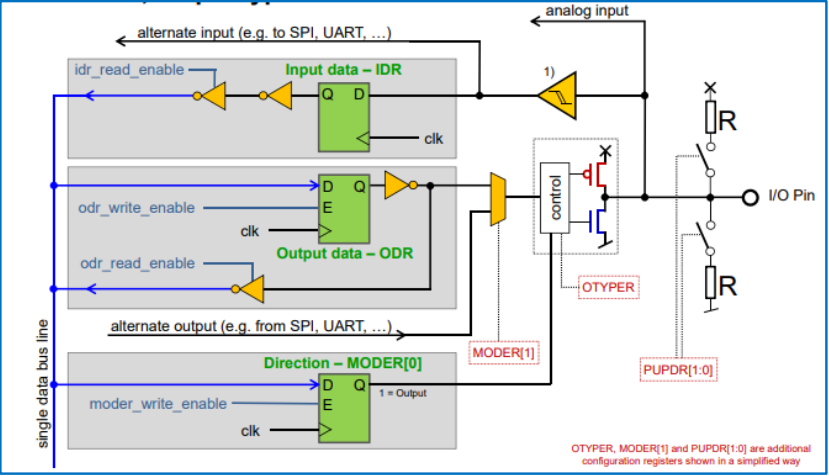
\includegraphics[width=\linewidth]{structure_gpio.png}
\end{concept}

\begin{theorem}{Configuration Registers}
    \begin{itemize}
        \item \textbf{GPIOx\_MODER} (Mode Register)
        \item \textbf{GPIOx\_OTYPER} (Output Type Register)
        \item \textbf{GPIOx\_OSPEEDR} (Output Speed Register)
        \item \textbf{GPIOx\_PUPDR} (Pull-up/Pull-down Register)
    \end{itemize}
    %TODO: Add more information
\end{theorem}

\begin{corollary}{Data Operations}
    \begin{itemize}
        \item Input: Read register \textbf{GPIOx\_IDR} (Input Data Register)
        \item Output: Write register \textbf{GPIOx\_ODR} (Output Data Register) or \textbf{GPIOx\_BSRR} (Bit Set Reset Register)
    \end{itemize}
\end{corollary}

\begin{KR}{Setting and Clearing Bits} GPIOx\_BSRR
    \begin{itemize}
        \item 0-15: Set Bits $\rightarrow$ 1: Set, 0: No Change
        \item 16-31: Reset/Clear Bits $\rightarrow$ 1: Reset, 0: No Change
        \item Ensures atomic access in software (no interruption possible)
    \end{itemize}
\end{KR}

\begin{definition}{Configuration}
    %TODO: Add more information!!
    \begin{itemize}
        \item \textbf{Mode:} Input, Output, Alternate Function, Analog
        \item \textbf{Type:} Push-Pull, Open Drain
        \item \textbf{Speed:} Low, Medium, High, Very High
        \item \textbf{Pull-Up/Pull-Down:} No, Pull-Up, Pull-Down, Reserved
    \end{itemize}
\end{definition}

\begin{definition}{Hardware Abstraction Layer (HAL)}\\
    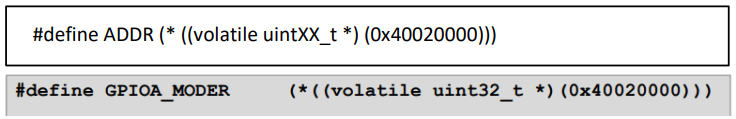
\includegraphics[width=\linewidth]{HAL1.png}\\
    \textbf{Accessing a register:}
    \begin{itemize}
        \item each GPIO port has the same 10 registers 
        \item there are 11 GPIO ports $\rightarrow$ GPIOA to GPIOI
    \end{itemize}
    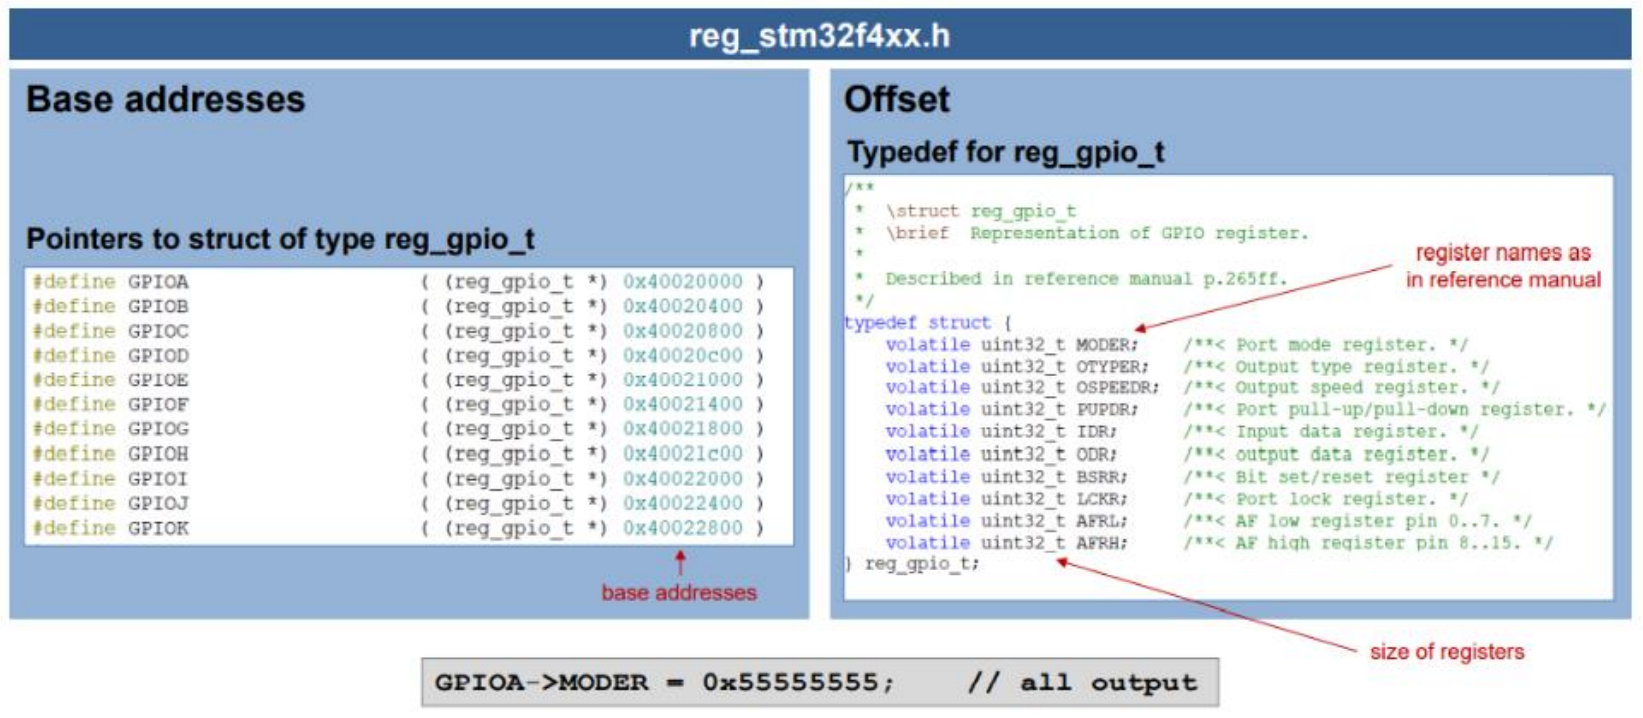
\includegraphics[width=\linewidth]{HAL2.png}
\end{definition}

\subsection{Conclusion}

\begin{KR}{Conclusion}
\end{KR}

\begin{remark}
    Learning Objectives:
    At the end of this lesson, you will be able
    - to work with register descriptions in reference manuals
    - to explain the concept and implementation of GPIOs
    - to explain the differences between open-drain and push-pull
    - to use GPIOs in your own programs
    - to explain the idea of a HAL
\end{remark}


